%-------------------------------------------------------------------------------
% TEMPLATE FOR UCL MSc THESIS
%------------------------------------------------------------------------------- 



% ------------------ DOCUMENT SETUP ------------------ 
% The document class defines the document type (report) and sets the font size (12pt)
\documentclass[12pt]{report}
\author{Your Name}


% Inputs the Document Packages
\input{_Packages}

% Controls how many subsections the document can take
%  and how many of those will get put into the contents pages.
\setcounter{secnumdepth}{3}
\setcounter{tocdepth}{3}

% Line Spacing
\setstretch{1.5}


% Places a dot after Chapter/Section/Subsection number in Table of Contents
\renewcommand{\cftchapaftersnum}{.}
\renewcommand{\cftsecaftersnum}{.}
\renewcommand{\cftsubsecaftersnum}{.}

%  Customize Dot spacing in Table of Contents/List of Figures/Tables
\renewcommand{\cftdotsep}{0.3}


% Line Break Properties
\tolerance=1
\emergencystretch=\maxdimen
\hyphenpenalty=10000
\hbadness=10000


% Formatting Table of Contents/Lists titles
\renewcommand{\contentsname}{\bfseries\LARGE{CONTENTS}}
\renewcommand{\listfigurename}{\bfseries\LARGE{LIST OF FIGURES}}

% Signature Line for the declaration
\newbox\namebox
\newdimen\signboxdim

\def\signature#1{%
    \setbox\namebox=\hbox{#1}
    \signboxdim=\dimexpr(\wd\namebox+3cm)
    \parbox[t]{\signboxdim}{%
        \centering
            \hrulefill\\    % for a line
            #1
        \par}%
    }

% Title Formatting customization
\titleformat{\chapter}{\normalfont\bfseries\LARGE}{\thechapter.}{1em}{\MakeUppercase}

\titleformat{\section}{\normalfont\bfseries\large}{\thesection.}{1em}{\MakeUppercase}
\titlespacing*{\section} {0pt} {0pt} {15pt} % left, before, after

\titleformat{\subsection}{\normalfont\bfseries\large}{\thesubsection.}{1em}{}
\titlespacing*{\subsection} {0pt} {10pt} {10pt}

\titleformat{\subsubsection}{\normalfont\bfseries\large}{\thesubsubsection.}{1em}{}
\titlespacing*{\subsubsection} {0pt} {10pt} {10pt}


% HEADER AND FOOTER
\pagestyle{fancy}  % Set Page Style (Header and Footer Style)
\fancyhf{}  % Clears the header and footer (from the default info)

% Header
\renewcommand{\headrulewidth}{0pt}  % Removes the default Horizontal Line in Header
% Optional Headers
%\fancyhead[L]{}
%\fancyhead[R]{2022/2023}

% Footer
\fancyfoot[C]{\thepage} % Page Number

% Change figure numbering per section
\numberwithin{figure}{chapter}

%Acronym entries
\makeglossaries
\newacronym{US}{US}{Ultrasound}



%  -------------------------------------------------
%  --------- The document starts from here --------- 
%  -------------------------------------------------

\begin{document}


% ------------------  TITLE PAGE -------------------
\begin{titlepage}
\begin{center}
    % UCL IMAGE
    \vspace*{-3cm}
    \makebox[\textwidth]{\includegraphics[width=\paperwidth]{Images/UCL_header.png}}
    
    \vspace{2.3cm}
    
    % Title
    {\relscale{1.19}{A thesis submitted in partial fulfilment of the requirements for the degree of Master of Science (MSc) in}}

    \vspace{1cm}
    {\relscale{1.15}\textbf{PHYSICS AND ENGINEERING IN MEDICINE\\}}
    \vspace{0.3cm}
    {\relscale{1.15}\textbf{UNIVERSITY COLLEGE LONDON\\}}
    \vspace{2.4cm}
    
    {\relscale{1.19}{TITLE}}\\
    %\vspace{0.1cm}
    By\\
    %\vspace{0.1cm}
    YOUR NAME\\
    \vspace{0.9cm}
    {\begin{singlespace}First Supervisor: \\
    Second Supervisor: \\\end{singlespace}}
\end{center}
{\raggedleft\vfill{\begin{singlespace}
     Department of Medical Physics\\
  and Biomedical Engineering\\
\end{singlespace}
 UNIVERSITY COLLEGE LONDON\\
 \begin{singlespace}
 Date of submission: \today\\
 Word count: WORD COUNT\\
 \end{singlespace}
}\par
}
\end{titlepage}


% ------------------  TABLE OF CONTENTS --------------------
\newpage
\tableofcontents 


% -------------------  INTRODUCTION  ---------------------
\chapter{Introduction}
\section{Background}
\blindtext \\

\section{Citation Example}
This is how you cite \cite{savitzky,Harvey2002}.\\

\section{Acronym examples}
\gls{US} is an example of acronym use.\\
\newpage
\section{Figure use}
Here is an example of a figure (Fig. \ref{fig:example}).\\

 \begin{figure}[!ht]
    \centering
    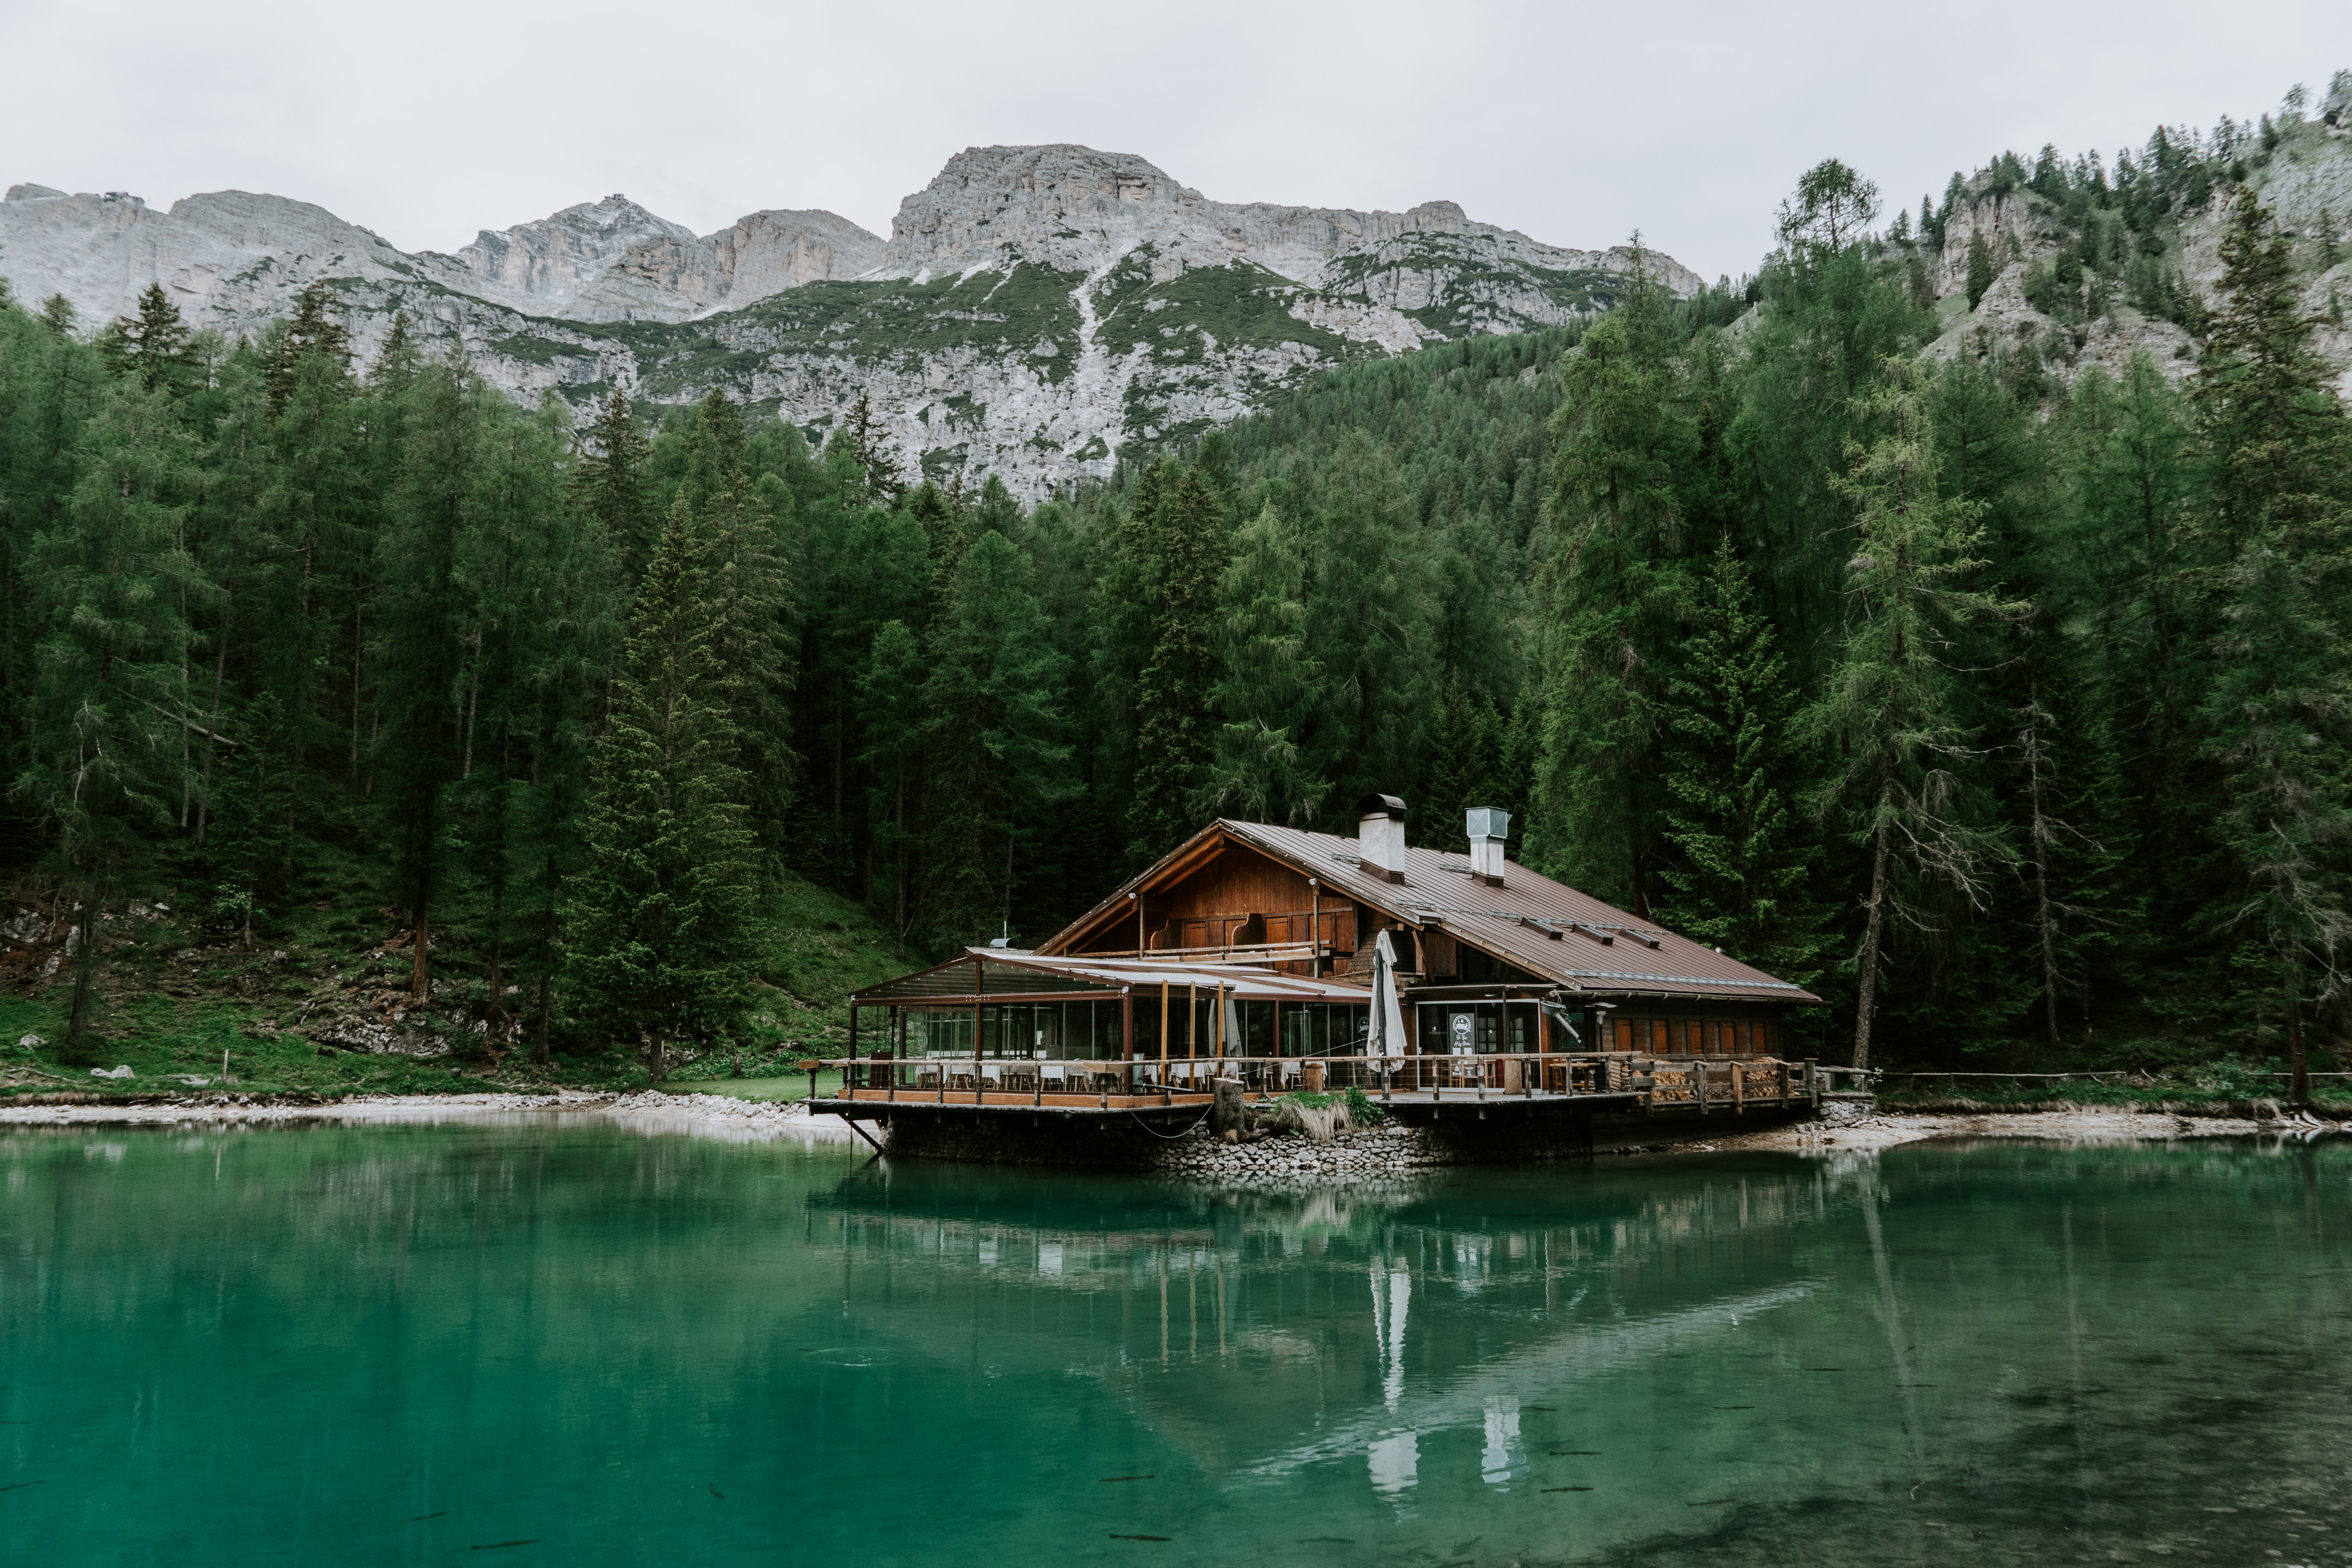
\includegraphics[width=0.9\textwidth]{Images/Stock_image.jpg}
    \caption{Example figure.}
    \label{fig:example}
\end{figure}
 % Section/Chapter entries can be done in the Main.tex file or in a  
                       % separate tex file for longer and more complex documents


% -------------------  MATERIALS AND METHODS  ---------------------
\chapter{Materials and Methods}
\section{Example 1}
\blindtext \\

\subsection{Example 1.1}
\blindtext \\

\subsubsection{Example 1.1.1}
\blindtext \\

\section{Example 2}
\blindtext % Section/Chapter entries can be done in the Main.tex file or in a  
                       % separate tex file for longer and more complex documents



% -------------------  RESULTS  ---------------------
\chapter{Results}
\input{Results} % Section/Chapter entries can be done in the Main.tex file or in a  
                       % separate tex file for longer and more complex documents

% -------------------  DISCUSSION  ---------------------
\chapter{Discussion}
\input{Discussion} % Section/Chapter entries can be done in the Main.tex file or in a  
                       % separate tex file for longer and more complex documents

                       
% -------------------  CONCLUSION AND FUTURE OUTLOOK  ---------------------
\chapter{Conclusion and Future Outlook}
\section{Conclusion}
\blindtext \\

\section{Future Outlook}
\blindtext % Section/Chapter entries can be done in the Main.tex file or in a  
                       % separate tex file for longer and more complex documents                       
% -------------------  BIBLIOGRAPHY ---------------------
\newpage
\bibliographystyle{elsarticle-num.bst}
\bibliography{References}
\addcontentsline{toc}{chapter}{References} % Adds References Section to Table of Contents
% -------------------  Appendix  ---------------------
\chapter*{Appendix}
\addcontentsline{toc}{chapter}{Appendix}
\section*{Appendix A}
\addcontentsline{toc}{section}{Appendix A}
\blindtext
\newpage
\section*{Appendix B}
\addcontentsline{toc}{section}{Appendix B}
\blindtext % Section/Chapter entries can be done in the Main.tex file or in a  
                       % separate tex file for longer and more complex documents                       

\end{document}
%  -------------------------------------------------
%  --------- The document ends from here ----------- 
%  -------------------------------------------------